\documentclass{custom}
\usepackage{graphicx} % Required for inserting images
\usepackage{setspace} % Required for line spacing
\usepackage{tocloft} % Required for table of contents
\usepackage{float} % Required for floating objects
\renewcommand{\cftchapleader}{\cftdotfill{\cftchapdotsep}}
\renewcommand{\cftchapdotsep}{\cftdotsep}
\usepackage{graphicx}
\usepackage{amsmath,amssymb}
\usepackage{tabularx}

\bibliographystyle{IEEEtran}


\pagestyle{empty}
\begin{document}

% Institute Logo and Name (same page as title)
\begin{center}
\includegraphics[width=1.5in]{logo.png}
\vspace{0.4cm}
{\large \textbf{\uppercase{\\Tribhuvan University}}}
\vspace{0.1cm}
{\large \textbf{\uppercase{\\Institute Of Engineering}}}
\vspace{0.1cm}
{\large \textbf{\uppercase{\\Thapathali Campus}}}
\vspace{2cm}
{\large \textbf{\\A Project Proposal}}
\vspace{0.1cm}
{\large \textbf{{\\on}}}
\vspace{0.1cm}
{\large \textbf{{\\Fine-Tuning of Llama-2 7B for Python Code Generation}}}
\vspace{2cm}
{\large \textbf{\\Submitted by:}}
{\large {{\\Deep Shrestha (THA079BCT011)}}}
\vspace{0.1cm}
{\large {{\\Pradip Pokhrel (THA079BCT027)}}}
\vspace{0.1cm}
{\large {{\\Rohan Dhakal (THA079BCT033)}}}
\vspace{0.1cm}
{\large {{\\Sanjay Shrestha (THA079BCT039)}}}
\vspace{2cm}
{\large \textbf{{\\Submitted to:}}}
{\large \\Department of Electronics and Computer Engineering}
{\large \\Thapathali Campus}
{\large \\Kathmandu, Nepal}
\vspace{2cm}
{\large {\\December 26, 2025}}

\end{center}
\chapter*{ACKNOWLEDGEMENT}
% No need for \addcontentsline; KOMA-script classes usually handle this 
% or the main.tex handles the TOC entry for the front matter.

\onehalfspacing % Matches the campus 1.5 line spacing requirement

We would like to express our sincere gratitude to the Department of Electronics and Computer Engineering, Thapathali Campus, and Asst. Prof. Suwarna Lingden, for his invaluable guidance, encouragement, and insightful feedback that greatly enhanced the quality of our work. We extend our heartfelt thanks to all those who have supported and guided us throughout the process of preparing this project proposal.

\vspace{1.5cm}

\noindent
\textbf{Submitted By:}\\
\authorTable 
% Using \authorTable ensures the names and roll numbers align perfectly 
% as defined in your .cls file.
\chapter*{ABSTRACT}
\addcontentsline{toc}{chapter}{ABSTRACT}
\begin{normaltext}
    Fine-tuning large language models requires intensive hardware resources, making full fine-tuning infeasible to train under low resources constraints. Although some large language models perform better in Python code generation but they are not feasible for training in custom datasets. Addressing this gap requires efficient fine-tuning that reduces memory and computation overhead. This project aims to fine-tune Llama-2 7B for python code generation by Parameter Efficient Fine Tuning (PEFT) with QLoRA, focusing on the hardware level constraints. The training dataset is constructed from multiple open-source repositories, including FlyTec, StaQC and Alpaca 18k. Preprocessing involves filtering non-Python samples, cleaning noisy code, and formatting the data into instruction–response pairs suitable for supervised fine-tuning. The fine-tuned model will be evaluated on unseen python problems. Performance will be compared with the base model Llama-2 7B to assess improvement achieved through fine-tuning Llama-2 7B. The Fine-tuned model is expected to be capable of generating python code solutions for common coding exercises, using mixture of common programming problems and LeetCode problems as a benchmark on low edge devices.
    
\vspace{18 pt}

\textit{Keywords: PEFT, QLoRA, LoRA, OPT, Hugging Face. }

\end{normaltext}


\tableofcontents
\newpage
\addcontentsline{toc}{chapter}{List of Figures}
\listoffigures
\newpage
\addcontentsline{toc}{chapter}{List of Tables}
\listoftables
\newpage
\addcontentsline{toc}{chapter}{List of Abbreviations}
\chapter*{List of Abbreviations}
\begin{normaltext}

\begin{tabularx}{\textwidth}{@{}>{\bfseries}l@{:\ }X@{}}
BLEU  & Bilingual Evaluation Understanding \\
CoT   & Chain-of-Thought \\
DVC   & Data Version Control \\
GPT   & Generative Pre-trained Transformer \\
GPUs  & Graphics Processing Units \\
IDE   & Integrated Development Environment \\
LLaMA & Large Language Model Meta AI \\
LLM   & Large Language Model \\
LoRA  & Low-Rank Adaptation \\
NF4   & 4-bit NormalFloat \\
OPT   & Open Pre-trained Transformer \\
PEFT  & Parameter-Efficient Fine-Tuning \\
QLoRA & Quantized Low-Rank Adaptation \\
VRAM  & Video Random Access Memory \\


\end{tabularx}
\end{normaltext}
\setcounter{chapter}{0}
\chapter{Introduction}
\section{Background}
Advent of LLM have fundamentally changed the software development and code
writing process. LLM have become integral part of the workflow for developers and students. Even with this much of success, LLMs rely on massive datasets and big GPUs for training and running these models which makes them impossible for student and general people to run and train locally.

Fine-tuning is the process of further training a pre-trained LLM on a smaller, task-specific dataset. While the initial pre-training gives universal linguistic knowledge, fine-tuning shapes this generalized competence into specialized expertise.

The OPT-350M (Open Pre-trained Transformer) model, developed by Meta AI, is a
decoder-only LLM. With its 350 million parameters, it gives an important balance. It is large enough to possess meaningful generative capacity, yet small enough to be computationally efficient for research, development, and fine-tuning on consumer-grade or limited-resource hardware. This makes it an ideal candidate for demonstrating efficient specialization techniques.

\section{Objectives}
A. Making better code generator than existing OPT-350M by finetuning it on python code datasets.
\\
B. Using PEFT through QLoRA to finetune base model i.e OPT-350M.
\chapter{LITERATURE REVIEW}
\begin{normaltext}
\vspace{18pt}
\section{Transformer Architecture and Attention Mechanism}
The foundation of modern large language models is built on the Transformer architecture introduced by Vaswani et al. \cite{Vaswani2017}. The "Attention Is All You Need" paper presents the self-attention mechanism and encoder-decoder architecture that forms the basis for contemporary LLMs. This revolutionary approach has become the de facto standard for natural language processing tasks and remains the core architecture for models discussed in this review.

\vspace{18pt}
\section{Scaling Laws and Transfer Learning}
Understanding the scaling properties of neural language models is crucial for efficient model development. Kaplan et al. \cite{Kaplan2020Scaling} established fundamental scaling laws for neural language models, providing insights into how model performance improves with increased parameters, training data, and computational resources. Additionally, Howard and Ruder \cite{Howard2018ULMFiT} introduced Universal Language Model Fine-tuning (ULMFiT), demonstrating that transfer learning from pre-trained models can achieve state-of-the-art results on text classification tasks with limited labeled data. These foundational works highlight the effectiveness and efficiency of fine-tuning approaches.

\vspace{18pt}
\section{Few-Shot Learning and In-Context Learning}
Brown et al. \cite{Brown2020} demonstrated that large language models exhibit remarkable few-shot learning capabilities, introducing GPT-3 and showing that models with sufficient scale can perform new tasks from just a few examples without explicit parameter updates. This capability has become fundamental to understanding how LLMs can be adapted for various downstream tasks.

\vspace{18pt}
\section{Parameter-Efficient Fine-Tuning (PEFT)}
Beyond LoRA and QLoRA, parameter-efficient approaches have gained significant attention. Houlsby et al. \cite{Houlsby2019} introduced parameter-efficient transfer learning for NLP through adapter modules, demonstrating that significant performance can be achieved by training only a small fraction of parameters. More recently, Liu et al. \cite{Liu2024DoRA} proposed DoRA (Weight-Decomposed Low-Rank Adaptation), which decomposes weight matrices into magnitude and direction components, providing further improvements over standard LoRA in various tasks.

\vspace{18pt}
\section{Low Rank Adaptation (LoRA)}
Hu et al.\cite{Hu2021} introduced LoRA, which freezes pre-trained model weights and injects trainable rank decomposition matrices into each Transformer layer. This approach reduces trainable parameters by 10,000 times and GPU memory requirements by 3 times compared to full fine-tuning of GPT-3 175B, enabling efficient adaptation on modest hardware without significant performance degradation.

\vspace{18pt}
\section{Quantized Low-Rank Adaptation (QLoRA)}
Dettmers et al.\cite{Dettmers2023} extended LoRA by combining quantization with low-rank adaptation. QLoRA introduces 4-bit NormalFloat (NF4), Double Quantization, and Paged Optimizers to achieve further memory reduction. This approach achieved 99.3\% of ChatGPT's performance with only 24 hours of single-GPU training, demonstrating that small, high-quality datasets are sufficient for state-of-the-art results when paired with efficient fine-tuning techniques.

\vspace{18pt}
\section{Open LLMs}
Many Large Language Models have been released for public use and for research purpose. Zhang et al. \cite{Zhang2022} released Open Pre-trained Transformers (OPT), a suite of decoder-only pre-trained models ranging from 125M to 175B parameters with full model weights made publicly available. The OPT models does not work well with declarative instructions or point-blank interrogatives \cite{Zhang2022}. Touvron et al. \cite{Touvron2023Llama2} introduced Llama 2, a family of pre-trained and fine-tuned LLMs ranging from 7B to 70B parameters. Llama 2 models outperform open-source models of similar size and are competitive with proprietary models like GPT-3.5 and PaLM 2 on various benchmarks. With its larger training dataset and superior architecture, Llama 2 demonstrates strong capabilities in code generation tasks compared to earlier models like OPT. Diehl et al. \cite{Diehl2024Llama2Benchmark} conducted comprehensive benchmarking of Llama-2 70B across multiple programming languages, evaluating its capabilities in code generation, documentation, translation, and unit test creation. Their findings reveal that while the model performs well on simpler numerical tasks, it faces substantial challenges with complex, parallelized, or distributed computations, requiring significant manual corrections for production-ready code.

\vspace{18pt}
\section{Domain-Specific Application}
The practical effectiveness of Parameter Efficient Fine-Tuning (PEFT) techniques is demonstrated in fine-tuning CodeLlama-7B for Fortran code generation \cite{Govande2024}. Using LoRA to adapt only attention weights while freezing MLP modules, the researchers fine-tuned the model on high-quality Fortran code from public repositories and NASA codebases, with GPT-3.5 generated descriptions. The fine-tuned model significantly outperformed vanilla CodeLlama-7B-Instruct, achieving 41\% improvement in compilation rate, 150\% improvement in execution rate, and 75\% improvement in correct output rate on 540 LeetCode problems.

\vspace{18pt}
\section{Chain-of-Thought and Code Generation}
Li et al. \cite{Li2023CoTCodeGen} explored chain-of-thought prompting techniques for code generation, demonstrating how decomposing complex programming tasks into step-by-step reasoning improves model performance. This approach has proven valuable in enhancing code quality and correctness when generating code solutions.

\vspace{18pt}
\section{Evaluation Metrics for Code Generation}
Proper evaluation of generated code is critical for assessing model performance. Papineni et al. \cite{Papineni2002} introduced BLEU (Bilingual Evaluation Understanding), a widely-used automatic evaluation metric for machine translation and code generation tasks. While BLEU provides a standardized measurement, additional metrics specific to code compilation and execution are often necessary for comprehensive evaluation.

\vspace{18pt}
\section{Training with Noisy Labels}
Zhang and Sabuncu \cite{Zhang2018GCE} proposed Generalized Cross Entropy Loss for training deep neural networks with noisy labels. This technique is relevant when training on synthetic or imperfect code datasets, where maintaining robustness against label noise is essential for model reliability.



\end{normaltext}

\chapter{METHODOLOGY}
This project aims to fine-tune the Llama-2 7B large language model for Python code generation. The methodology is structured into three distinct phases: dataset preparation, model fine-tuning, and performance evaluation.

Figure~\ref{fig:finalmodel} illustrates the system block diagram, while Figure~\ref{fig:decoder} provides a detailed view of the decoder block with the integrated QLoRA adapter.



\begin{figure}[H]
    \centering
    \includegraphics[width=0.65\linewidth]{model.jpg}
    \caption{System Block Diagram}
    \label{fig:finalmodel}
\end{figure}

\begin{figure}[H]
    \centering
    \includegraphics[width=0.85\linewidth]{decoder.jpg}
    \caption{Decoder Block Diagram with QLoRA Adapter}
    \label{fig:decoder}
\end{figure}

The architecture follows a decoder-only Transformer design. Input text is converted into embeddings and combined with positional encodings before entering a stack of 32 decoder layers (for Llama-2 7B). Within each layer, data passes through RMSNorm and a multi-head self-attention mechanism. Crucially, the QLoRA adapters are injected into the linear projections of the attention and Feed-Forward Network (FFN) blocks. This allows for task-specific parameter updates while keeping the base model's 4-bit quantized weights frozen.

\section{Dataset Description and Preparation}
Fine-tuning for Python code generation requires a high-quality dataset containing diverse programming tasks. We construct a composite dataset from multiple open-source repositories.

\subsection{Dataset Sources and Composition}
\begin{table}[H]
    \centering
    \caption{Dataset Sources and Composition}
    \begin{tabularx}{\textwidth}{|>{\bfseries}l|X|X|l|}
        \hline
        \textbf{Dataset} & \textbf{Size} & \textbf{Content \& Reason} & \textbf{License} \\ \hline
        FlyTech Python & $\sim$42,000 pairs & Python scripts with structured tasks and docstrings. & MIT \\ \hline
        Alpaca-18k & $\sim$18,000 pairs & Instruction prompts for prompt diversity. & CC BY-NC \\ \hline
        LeetCode & 200--300 & Competitive tasks for functional testing. & Fair use \\ \hline
    \end{tabularx}
    \label{tbl:datasets}
\end{table}

\subsection{Dataset Processing Pipeline}
The collected data undergoes a rigorous preprocessing pipeline:
\begin{itemize}
    \item \textbf{Duplicate Removal:} Eliminating identical instruction–code pairs to prevent overfitting.
    \item \textbf{Syntactic Filtering:} Discarding incomplete or syntactically incorrect Python code using AST parsing.
    \item \textbf{Chain-of-Thought (CoT) Enrichment:} Adding step-by-step reasoning to help the model learn logical structure.
    \item \textbf{Normalization:} Standardizing indentation (PEP 8) and naming conventions.
\end{itemize}



\begin{table}[H]
    \centering
    \caption{Final Expected Dataset Size}
    \begin{tabular}{l r}
        \textbf{Source} & \textbf{Count} \\ \hline
        FlyTech & $\sim$40,000 \\
        Alpaca & $\sim$17,000 \\ \hline
        \textbf{Total Usable Examples} & \textbf{$\sim$57,000} \\
    \end{tabular}
\end{table}

\subsection{Instruction Formatting and Tokenization}
Each example is formatted into an instruction-style structure. For example:
\begin{quote}
\texttt{Instruction:} Write a Python code for printing whether a given number is Armstrong.\\
\texttt{Chain of thought:} [Logical steps...]\\
\texttt{Response:} [Python Code Block]
\end{quote}

\section{Model Fine-Tuning}
The model utilizes the instruction-tuning paradigm. Given a prompt $x$, the model predicts the target token sequence $y$ by maximizing the likelihood:
\begin{equation}\label{eq:loss}
\mathcal{L} = -\sum_{t=1}^{T} \log P_{\theta} (y_{t} \mid y_{<t}, x)
\end{equation}

\subsection{QLoRA for Efficient Training}
QLoRA achieves efficiency by freezing the 4-bit quantized base weights and optimizing only the low-rank adapter matrices. This reduces the VRAM requirement to approximately 16GB, fitting within the constraints of an NVIDIA RTX 3060 or Google Colab T4.

\begin{figure}[H]
    \centering
    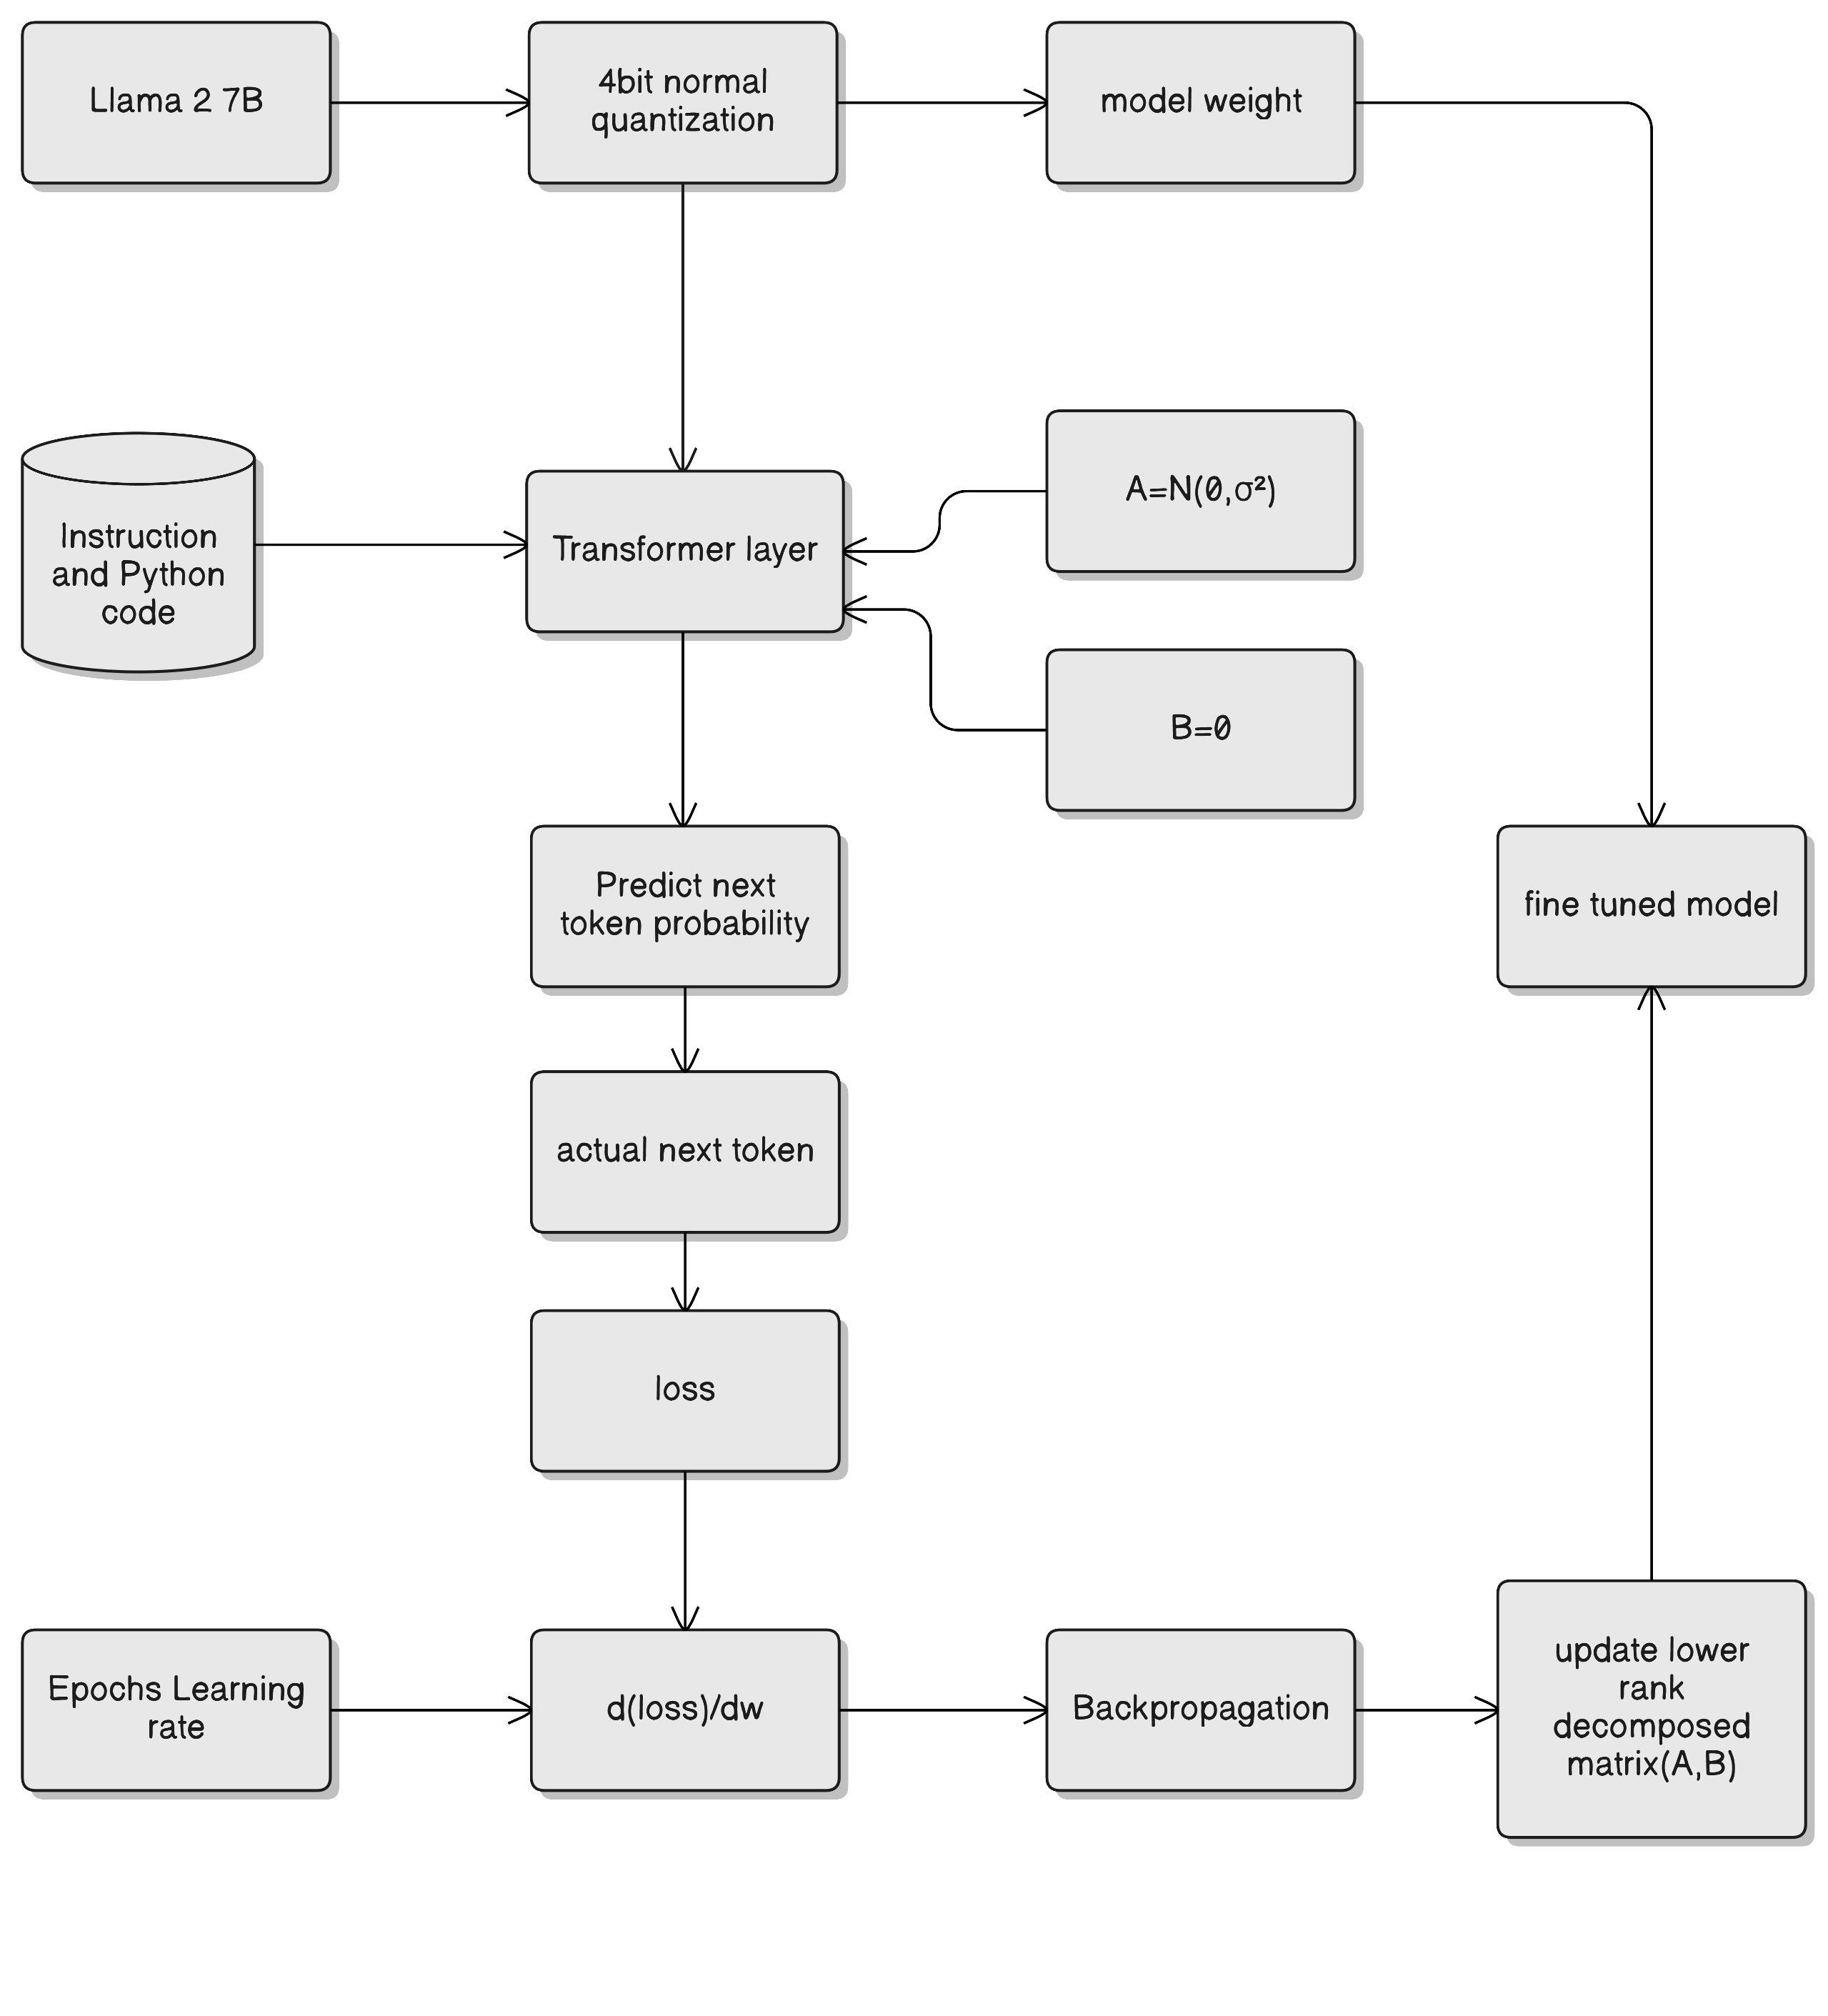
\includegraphics[width=1\linewidth]{flowdiagram.png} 
    \caption{Base Model Fine-tuning with QLoRA Adapter Layers}
    \label{fig:qlora_flow}
\end{figure}

\section{Evaluation Metrics}
Evaluation is split into functional correctness and similarity-based metrics.

\subsection{Functional Correctness}
Generated solutions are executed in a secure Docker sandbox and classified as:
\begin{itemize}
    \item \textbf{Right:} Passes all test cases.
    \item \textbf{Partial:} Passes some test cases.
    \item \textbf{Wrong:} Fails output or crashes.
\end{itemize}

\subsection{Automatic Similarity Metrics}
We utilize BLEU and CodeBLEU for quantitative assessment. CodeBLEU integrates structural information via Abstract Syntax Trees (AST) and data-flow:
\begin{equation}
\text{CodeBLEU} = \alpha \cdot \text{BLEU} + \beta \cdot \text{AST} + \gamma \cdot \text{DFScore} + \delta \cdot \text{SemanticScore}
\end{equation}
where $\alpha, \beta, \gamma, \delta$ are weighted parameters.
\chapter{Expected Outcome}

\begin{normaltext}This model is expected to generate python code based on the provided textual prompt
using OPT-350M. The fine-tuned model is expected to achieve higher accuracy than OPT-350M in python code generation specific domain which is expected to answer with higher accuracy to LeetCode problems. This model also focuses
on human readability by providing extra comments and docstring wherever required.
\vspace{18 pt}

The fine-tuned model will be runnable in low specification devices with higher
accuracy than the previous model and A common end goal in the field of code
generation is to generate functional and deployable end-to-end systems that can be used
in real-world settings.

\end{normaltext}
\chapter{PROJECT SCHEDULE}

% Tip: adjust the timeline and tasks below to match your plan.
% Use exact dates for tasks; calendar shows only months
\begin{table}[H]
	\centering
	\caption{Project schedule (Gantt chart)}
	\includegraphics[width=1\textwidth]{Planning.png}
	\label{fig:project_schedule}
\end{table}
\chapter{FEASIBILITY ANALYSIS}

This project is primarily targeted at fine-tuning large language models for Python code generation using Parameter Efficient Fine-Tuning (PEFT) with QLoRA. The feasibility of this project is analyzed from the following perspectives:

\section*{Operational Feasibility}
The project is designed to be applicable on relatively low-end devices. The hardware requirement for Llama-2 7B is approximately 6-8GB of VRAM, which is widely available in consumer-grade GPUs such as the NVIDIA RTX 3060 or 4060, as well as the Google Colab free tier (T4 GPU). 



The use of QLoRA significantly reduces the memory footprint, making it feasible to execute fine-tuning on a single consumer-grade GPU rather than requiring an enterprise-level server cluster.

\section*{Economic Feasibility}
The project utilizes freely available open-source models (Llama-2) and public datasets (FlyTec, StaQC). Since the hardware constraints are low enough to utilize existing consumer-grade GPUs or free cloud-based services like Google Colab, the primary development cost is zero. If extended training time is required beyond the free tier limits, Google Colab Pro can be utilized at a nominal cost of approximately \$10 per month.

\section*{Technical Feasibility}
The implementation relies on well-established, industry-standard libraries such as Hugging Face \texttt{transformers}, \texttt{peft}, and \texttt{bitsandbytes}. These libraries provide robust support for 4-bit quantization and LoRA adapter integration. The team possesses the necessary proficiency in Python programming and machine learning frameworks to manage the model loading, data preprocessing, and evaluation pipelines effectively.
\nocite{*}
\bibliography{references}
\end{document}